\documentclass[12pt]{article}

\usepackage{sbc-template}
\usepackage{graphicx,url}
\usepackage[brazil]{babel}
\usepackage[utf8]{inputenc}
\usepackage{float}
\usepackage{setspace}

\usepackage{tabularx}
\usepackage{cite}

\begin{document}
\sloppy

\title{Comunidade.UnB - Um estudo de caso de implantação e \\
    desenvolvimento de software livre na universidade.}

\author{Carlos Denner\inst{1}, Daniel C. Bucher\inst{2}, Paulo R. M. Meirelles\inst{2},  Wilton Rodrigues\inst{2}}


\address{Departamento de Administração -- Universidade de Brasília (UnB)\\
  Campus Universitário Darcy Ribeiro - ICC Ala Norte, Bloco B -- Brasília -- DF -- Brasil
\nextinstitute
  Faculdade do Gama -- Universidade de Brasília (UnB)\\
  Área Especial, Projeção A -- 72.444-240 -- Gama -- DF -- Brasil
\email{\{carlosdenner,daniel.bucher88,braynwilton\}@gmail.com, paulo@softwarelivre.org}
}


\maketitle
\begin{abstract}
  Abstract.

\textbf{Keywords:} free software, etc.

\end{abstract}

\begin{resumo}
  Resumo.

\textbf{Palavras-chave:} \textit{software} livre, etc.
\end{resumo}


%-----------------------------------------------------------------------------%
\section{Introdução} \label{sec:intro}

Este artigo apresenta os resultados de um estudo de caso de implantação e
desenvolvimento de software livre na Universidade de Brasília (UnB). O
software livre em questão é o Noosfero\footnote{\url{http://noosfero.org/}},
uma plataforma para a criação de redes sociais livres criada pela
Cooperativa de Tecnologias Livres - Colivre%
\footnote{\url{http://colivre.coop.br/}}, uma empresa cooperativa que atua
exclusivamente com soluções livres. As contribuições para a comunidade do
Noosfero são feitas por alunos do Laboratório Avançado de Produção,
Pesquisa e Inovação em Software (LAPPIS)%
\footnote{\url{http://fga.unb.br/lappis/}} da UnB Gama desde junho de 2013
e produziram como resultado a implantação e a manutenção de dois ambiente
Noosfero na universidade: (\textit{i}) Comunidade.UnB\footnote{%
\url{http://comunidade.unb.br/}}, e o (\textit{ii}) Portal da UnB Gama%
\footnote{\url{http://fga.unb.br/}}. O primeiro é uma rede de colaboração
social para alunos, professores e funcionários técnico-administrativos da
UnB, ainda em estágio de homologação, e tem por objetivo fornecer um ambiente
virtual para a criação e o compartilhamento de conhecimento. O segundo é o
portal de informações e notícias da Faculdade do Gama (UnB/FGA).

Até a data da escrita deste artigo, os alunos do LAPPIS já contribuíram com
mais de vinte \textit{merge requests} incorporados no \textit{core} do
Noosfero e o Comunidade.Unb já possui 167 usuários e 24 comunidades.

%-----------------------------------------------------------------------------%
\section{Fundamentação Teórica} \label{sec:fundamentacao}

Nesta seção, apresentaremos o conceito de software livre e os motivos para
termos adotado ideologia no contexto deste artigo. Além disso, apresentaremos
a arquitetura e as principais características do Noosfero e do
\textit{framework} através do qual este foi desenvolvido, o
\textit{Ruby on Rails}.

%-----------------------------------------------------------------------------%
\subsection{Software Livre}

O princípio básico do ecossistema do software livre é promover a liberdade
do usuário, sem discriminar quem tem permissão para usar um software e seus
limites de uso, baseado na colaboração e num processo de desenvolvimento
aberto. Software livre é aquele que permite aos usuários usá-lo, estudá-lo,
modificá-lo e redistribui-lo, em geral, sem restrições para tal e prevenindo
que não sejam impostas restrições aos futuros usuários \cite{meirelles2013}.
Entendemos que este modelo de desenvolvimento de distribuição de software
seja o ideal em um estudo de caso envolvendo uma universidade, uma vez que
entendemos ser o papel da universidade não só promover a construção de
conhecimento, mas também a disseminação deste conhecimento para a sociedade,
e a utilização do software livre permite isso por causa dos quatro direitos
que este fornece%
\footnote{Extraído de \url{http://www.gnu.org/} em Julho de 2014}:

\begin{itemize}
  \item A liberdade de utilizar o software, para qualquer propósito;
  \item A liberdade de estudar como o software funciona e adaptá-lo para suas necessidades;
  \item A liberdade de redistribuir cópias para seus vizinhos;
  \item A liberdade de aprimorar o software, e redistribuir seus aprimoramentos para o público,
  de forma a beneficiar toda a comunidade;
\end{itemize}

%-----------------------------------------------------------------------------%
\subsection{Noosfero}

Noosfero é uma plataforma web livre para criação de redes sociais,
desenvolvida pela Cooperativa de Tecnologias Livres - Colivre, em 2007, sob
licença AGPLv.3, com a proposta de permitir aos usuários criarem sua própria
rede social personalizada, livre e autônoma.

O Noosfero foi desenvolvido na linguagem de programação Ruby%
\footnote{\url{http://www.ruby-lang.org/en/}},
versão 1.8.7, e utiliza o \textit{framework} Model-View-Controller (MVC) para
aplicações web Ruby on Rails%
\footnote{\url{http://rubyonrails.org/}}, versão 2.3.5.
%
A escolha destas tecnologias, por parte dos criadores do Noosfero, que também
trabalhamos juntos no contexto deste trabalho,
foi baseada no fato de que o Ruby possui uma sintaxe
simples, elegante e de fácil leitura, o que aumenta a manutenibilidade do sistema,
uma característica importante num projeto de software livre que visa atrair
desenvolvedores externos~\cite{meirelles2013}.
%
Outras características importantes que influenciaram essa escolha são a alta
capacidade produtiva que o \textit{framework} possui por priorizar conceitos como
\textit{convention over configuration} (convenção antes de configuração)
e DRY\footnote{Uma forma de apologia ao reuso de código}
(\textit{Don't Repeat Yourself} - Não Repita a Si Mesmo), bem como, o alinhamento
entre a comunidade do Ruby on Rails com metodologias ágeis de
desenvolvimento de software, que são evidenciadas em uma série de ferramentas que
viabilizam o uso de práticas como TDD\footnote{Desenvolvimento orientado a testes}
e BDD\footnote{Design orientado a comportamento}, práticas adotadas no
desenvolvimento do Noosfero, e neste trabalho.

Além disso, a arquitetura do Noosfero foi pensada para permitir que este seja facilmente
expansível, de forma que funcionalidades que não sejam comuns ao conceito de
redes sociais sejam desenvolvidas como \textit{plugins}, assim diminuindo
o acoplamento e aumentando a coesão dos diversos módulos do sistema.
%
Uma das grandes vantagens em se criar uma aplicação com arquitetura extensível
é a possibilidade de criar \textit{plugins} sem precisar modificar o código
fonte do núcleo da ferramenta, além de permitir o isolamento de \textit{bugs}
mais facilmente.

Essa abordagem arquitetural é muito benéfica para a diversidade de contextos
em que o Noosfero pode ser utilizado. Diversidade essa que pode ser evidenciada
quando se observa a existência de uma rede como o Cirandas%
\footnote{\url{https://cirandas.net/}},
uma rede social com o propósito de promover economia solidária através
da troca e venda de produtos e serviços, e o
Stoa, um ambiente virtual para a disseminação de conhecimento em âmbito
acadêmico de forma colaborativa, ambos desenvolvidos utilizando o Noosfero.
%
Dessa forma, os dois ambientes são instâncias do Noosfero que utilizam o seu
núcleo comum, mas diferem no uso de \textit{plugins} com funcionalidades
próprias às suas necessidades específicas.

\begin{figure}[H]
    \centering
      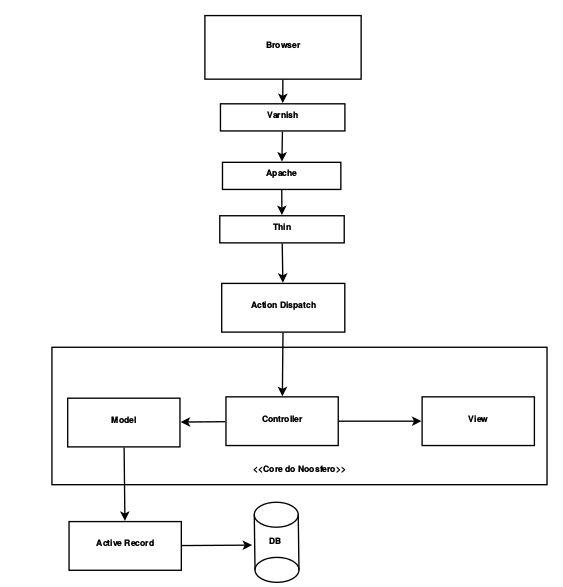
\includegraphics[keepaspectratio=true,scale=0.4]{images/noosfero-architecture.png}
    \caption{Visão arquitetural do Noosfero.}
    \label{noosfero-arch}
\end{figure}

A Figura \ref{noosfero-arch} apresenta uma visão arquitetural de alto nível
do núcleo do Noosfero. Vale a pena ressaltarmos alguns componentes desta arquitetura:

\begin{itemize}
    \item \textbf{Varnish:} acelerador de aplicações web também conhecido
    como cache de proxy reverso HTTP. É utilizado quando for necessário
    acessar conteúdo estático, imagens, \textit{scripts} e folhas de estilos.

    \item \textbf{Apache:} \textit{web-server} utilizado como servidor de
    \textit{proxy} reverso. Sua função é encaminhar as requisições que
    chegam para uma das instâncias do Thin.

    \item \textbf{Thin:} \textit{app-server} utilizado para processar as
    requisições de entrada e saída e encaminhá-las para o Noosfero para que
    ele possa executá-las. Pode ser configurado para utilizar mais de um
    processo para realizar balanceamento de carga. É recomendável o uso de
    dois processos do \textit{Thin} por núcleo de processador do servidor
    hospedeiro.

    \item \textbf{ActionDispatch:} funciona como roteador. Sua função é
    mapear as requisições que chegam a suas respectivas \textit{controllers}.

    \item \textbf{Controller:} controla o fluxo da aplicação. Realiza a
    ligação entre as entidades de \textit{model} e de \textit{view} através
    de chamadas de métodos.

    \item \textbf{Model:} representa as entidades do domínio da aplicação.
    A lógica da aplicação é implementado nas classes de \textit{model}.

    \item \textbf{View:} responsável pela visualização das páginas, isto é,
    as saídas em HTML da aplicação.

    \item \textbf{Active Record:} realiza o mapeamento entre os objetos de
    \textit{model} e o modelo relacional utilizado no banco de dados da
    aplicação.

\end{itemize}

%-----------------------------------------------------------------------------%
\section{Metodologia} \label{sec:metodologia}

A contribuição para a comunidade do Noosfero, no contexto do Comunidade.UnB e
do Portal da UnB Gama, é realizada por uma equipe de estagiários do LAPPIS,
assim como pela equipe do projeto do Novo Portal do Software Público%
\footnote{\url{http://www.participa.br/softwarepublico/}}, um projeto da UnB
em parceria com o Ministério do Planejamento, Orçamento e Gestão (MP). Nesta
seção apresentamos algumas práticas e metodologias utilizadas na evolução da
ferramenta. Na seção \ref{sec:resultados} apresentaremos
algumas funcionalidades desenvolvidas por nós de forma a adaptar o Noosfero
para o ambiente de uma universidade.

O processo de colaboração com o Noosfero inclui uma série de práticas apresentadas
pelas metodologias ágeis de desenvolvimento de software como o uso de testes
automatizados, a descrição das funcionalidades do projeto no formato de
histórias de usuário e a adoção de ferramentas para a utilização da metodologia
\textit{Behavior Driven Development} (BDD)%
\footnote{\url{http://en.wikipedia.org/wiki/Behavior-driven_development}},
uma evolução do \textit{Test Driven Development} (TDD)%
\footnote{\url{http://en.wikipedia.org/wiki/Test-driven_development}}
apresentada por \citeonline{north2006}.
%
As semelhanças das práticas adotadas pelas comunidades de software livre e as
comunidades de métodos ágeis foram apresentadas por \citeonline{corbucci2011}
em sua tese de mestrado. De acordo com ele, os dois
métodos possuem tantas características em comum ao ponto de, Martin Fowler,
um dos autores mais influentes na Literatura sobre métodos ágeis,
incluir software livre como um método ágil na primeira versão de seu artigo
\textit{"The New Methodology"}. No entanto, o mesmo foi retirado devido
à falta de descrição precisa dos métodos de desenvolvimento utilizados pelas
comunidades de software livre \cite{fowler2000}.

Por outro lado, \citeonline{corbucci2011} discute os princípios ágeis e livres
como semelhantes:
%
(\textit{i}) Indivíduos e interações são mais importantes que processos e
ferramentas;
(\textit{ii}) Software em funcionamento é mais importante que documentação
abrangente;
(\textit{iii}) Colaboração com o cliente (usuários) é mais importante que
negociação de contratos;
(\textit{iv}) Responder às mudanças é mais importante que seguir um plano.
%
Também, explicita as práticas disseminadas pelas metodologias ágeis usadas no
cotidiano dos desenvolvedores de software livre:
(\textit{i}) Código compartilhado (coletivo);
(\textit{ii}) Projeto simples;
(\textit{iii}) Repositório único de código;
(\textit{iv}) Integração contínua;
(\textit{v}) Código e teste;
(\textit{vi}) Desenvolvimento dirigido por testes, e
(\textit{vii}) Refatoração~\cite{corbucci2011}. Portanto, neste trabalho,
entendemos software livre como um método ágil de desenvolvimento, do ponto de
vista da Engenharia de Software.

\begin{figure}[h]
	\centering
	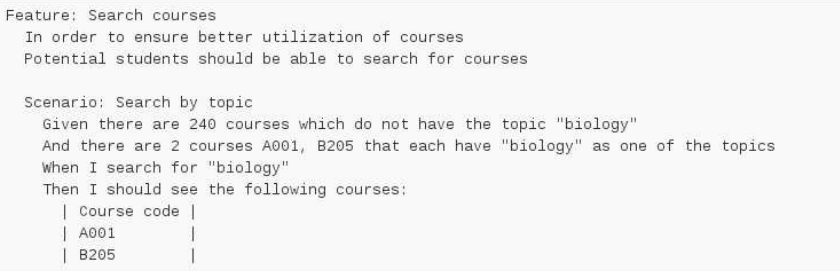
\includegraphics[keepaspectratio=true,scale=0.6]{images/cucumber-sample.png}
	\caption{Exemplo de utilização do cucumber}
	\label{cucumber}
\end{figure}

Para especificarmos as funcionalidades desenvolvidas por nós, utilizamos
o formato de Histórias de Usuários (\textit{User Stories}),
prática bastante difundida dentro das comunidades de métodos ágeis e também
adotada em algumas comunidades de software livre.
%
Além das histórias, utilizamos também o formato de critérios de aceitação
apresentados por \citeonline{north2006}, outra
prática ágil que vem ganhando força com a popularização do BDD.
%
O formato adotado é conveniente para nós, uma vez que o Noosfero utiliza o
\textit{cucumber}\footnote{\url{http://cukes.info/}}, uma ferramenta para
automatização de testes escritos em linguagem natural, criada para apoiar a
utilização de BDD. No \textit{cucumber}, os testes são escritos no formato
de funcionalidades e cenários, utilizando os formatos de histórias de
usuário e de critérios de aceitação mencionados. A Figura
\ref{cucumber}\footnote{Extraído de \url{https://github.com/cucumber/cucumber/wiki}}
apresenta um exemplo de uso do \textit{cucumber}.

O processo de desenvolvimento de software utilizado durante este trabalho
também se baseia em metodologias ágeis, com a utilização de ciclos curtos de
forma a permitir que haja \textit{feedback} de forma mais rápida e reuniões
curtas periodicamente na qual os integrantes da equipe apresentam o andamento
das funcionalidades previstas para aquele ciclo e os impedimentos encontrados.

%-----------------------------------------------------------------------------%
\section{Resultados} \label{sec:resultados}

Como resultado deste trabalho, a UnB possui hoje duas instâncias de Noosfero,
o Portal da UnB Gama, já em produção e o Comunidade.UnB, uma rede de colaboração
livre para os integrantes da universidade, ainda em processo de homologação,
além de uma série de \textit{patchs} submetidos e aceitos pelos mantenedores
oficiais do Noosfero. Nesta seção apresentamos algumas funcionalidades
desenvolvidas por nós para melhor adequar o Noosfero ao contexto da UnB.

A primeira funcionalidade desenvolvida surgiu da necessidade de se ter sub-%
comunidades para cada projeto da disciplina de Manutenção e Evolução de
Software da FGA, ministrada pelo Prof. Paulo Meirelles. O Noosfero já possuia
um \textit{plugin} que adicionava a possibilidade de criamos sub-comunidades
de determinada comunidade, no entanto este não oferecia uma forma clara do
usuário visualizar a relação entre estas. Como primeira colaboração deste
trabalho, desenvolvemos uma camada de visualização, dentro de uma comunidade,
na qual o usuário pudesse visualizar todas as comunidades ``filhas'' ou todas
as comunidades ``pais'' desta, uma vez que a relação entre comunidade e sub-%
comunidade é de N para N. Esta contribuição pode ser visualizada na comunidade
da disciplina mencionada%
\footnote{\url{http://comunidade.unb.br/profile/mes-fga/plugin/sub_organizations%
/children?display=full&type=community}}.

Outra contribuição interessante pro contexto da UnB, foi a melhoria no
\textit{plugin} de submissão de trabalhos, uma demanda que surgiu da
necessidade de existir um sistema web no qual os alunos pudessem enviar
seus trabalhos de conclusão de curso (TCC) e notificar seus orientadores e outros
interessados a respeito. Este \textit{plugin} permite não só que os alunos
façam upload de um arquivo, mas também que o mesmo seja versionado, criando
uma nova versão para cada novo upload realizado pelo mesmo aluno, além de
permitir a possibilidade de notificar pessoas interessadas via e-mail.
No primeiro semestre de 2014, foi realizado um teste%
\footnote{\url{http://fga.unb.br/tcc}} com os alunos do curso de engenharia de
software da FGA que estivessem fazendo TCC.

A \textit{wiki} do Participa.Br%
\footnote{\url{https://gitlab.com/participa/noosfero/wikis/CodeReview}},
um projeto de uma rede social livre para
possibilitar a participação social no meio virtual desenvolvido pela
presidência da república e que também contou com a contribuição dos alunos
do LAPPIS, possui uma série de \textit{patchs} (ou \textit{merge requests}
enviados no contexto deste trabalho, e de outros projetos do laboratório, e
já incorporado no núcleo do Noosfero.

%-----------------------------------------------------------------------------%
\section{Conclusão} \label{sec:conclusao}


Conclusão.

\bibliographystyle{sbc}
\bibliography{comunidade-unb}
\end{document}
